\chapter{I Was Bankrupt\ldots{} Now I've Made \$3 Billion}

This chapter follows Lecture 72 in School of Hard Knocks, curated by LazyingArt LLC. We should read it not as a blackboard lecture but as an interview whose mathematics lives inside commercial judgment: target and outcome, gross versus net, reinvestment, leverage, distribution, and the discipline of acting only on what can be controlled. The lecture begins with a compressed promise of scale, rewinds into biography, and then moves through a deliberate sequence: first identify what truly makes money, then understand sales as the great practical equalizer, then learn how patience, delegation, and debt can turn income into durable wealth.

\section{Opening Thesis: Belief Before Proof}

The interview opens with a teaser rather than with an explanation. Sean gives us the claim before the proof: on the first bid, before any policy had been sold, he promised a billion dollars in ten years. Then he gives us the realized number, not as a correction of the promise but as evidence of the kind of ambition he thinks business requires. We are meant to feel the scale first and ask questions afterward.

\paragraph{Anecdote.}
The opening number pair is simple and memorable:
\begin{align}
G_{10} &= \$1{,}000{,}000{,}000,\\
R_{10} &\approx \$800{,}000{,}000.
\end{align}
If we form the obvious ratio, we get
\begin{equation}
\frac{R_{10}}{G_{10}} \approx 0.8.
\end{equation}

\begin{remark}
This ratio is editorial rather than lecture-native. Sean does not present it as a formal metric. Still, it is a useful way to see the structure of the claim: the goal sounded absurd at the start, but even partial attainment was enormous.
\end{remark}

\paragraph{Claim.}
The lecture insists on a particular order. First one declares an ambitious future, then one works toward it, and only later does the world decide whether the original claim was delusional or prophetic. This is the business analogue of setting a boundary condition before the full trajectory is visible.

\paragraph{Mechanism.}
The opening is immediately complicated by a second claim: early money might have ruined him. The lecture therefore does not equate speed with wisdom. A million dollars at twenty-two is presented not as a pure blessing but as a destructive force in the wrong character and the wrong life-stage. The governing tension is set at once: belief matters, but timing and discipline matter too.

\section{From Broke Background to Revenue-Generating Focus}

After the teaser, the lecture resets into ordinary interview time. Sean places himself in Connecticut, in poverty, then in college athletics, state work, real estate, and later multiple businesses. This biographical sequence matters because it gives the later rules a social origin. He is not speaking from inherited capital or from a single polished career track.

\paragraph{Anecdote.}
One quantitative anchor from this part of the lecture is his description of working as a social worker for abused and neglected children:
\begin{equation}
S_{\text{social work}} = \$58{,}000/\text{year}.
\end{equation}
That figure matters because it sharpens the later point about wanting to provide more for his family and community without treating money as the original motive.

\paragraph{Claim.}
The first serious entrepreneurial question is not whether one is an ``expert,'' nor whether one is ``diversified.'' The first serious question is: which activity actually makes money? That is why Sean repeatedly demands paper. Lifestyle theater, gross activity, or being seen on a jet do not settle the matter.

\begin{definition}[Profitability Filter]
When several lines of activity coexist, the first one to back heavily is the one that survives inspection by the paper trail: the P\&L, the net figure, and EBITDA. Revenue alone is not enough.
\end{definition}

\begin{table}[h]
\centering
\begin{tabular}{|l|l|l|}
\hline
Measure & What it shows & Why it matters here \\
\hline
Revenue & gross movement & can be large even when the business is weak \\
\hline
Net & bottom-line earnings & tells us whether money remains after expenses \\
\hline
EBITDA & operating earnings proxy & tests the operating core before other items \\
\hline
Equity & ownership accumulated & points to future wealth, not just current pay \\
\hline
\end{tabular}
\caption{The documentary test Sean asks entrepreneurs to meet.}
\end{table}

\paragraph{Mechanism.}
If nine things are being done and only one of them produces real economics, then concentration is not a romantic choice. It is a bookkeeping consequence. The lecture's hostility to premature diversification is therefore not abstract. It is an attack on dilution of effort before the profitable line has been identified.

We may summarize the delayed-gratification logic that follows in a compact update chain:
\begin{equation}
\text{cash flow}_t \longrightarrow \text{reinvestment}_t \longrightarrow \text{capacity}_{t+1} \longrightarrow \text{cash flow}_{t+1}.
\end{equation}
Sean's language is concrete rather than theoretical: money came in, and it went back into the business. The businesses were ``eating,'' and therefore they were growing.

\subsection{Question \& Answer}

The lecture now raises a genuine local obstacle. Should one follow passion, or should one follow the thing that pays?

The answer is conditional. A young person without dependents has far more room to search. One may pursue what one wants, experiment, and even tolerate inefficiency for a while. But once family obligations exist, the lecture becomes much harder: cash flow is no longer optional. In that case, one may have to do things one does not love in order to purchase later freedom.

The important point is that Sean refuses sloganized advice. ``Follow your passion'' is not wrong in every case, and ``just chase money'' is not right in every case. The interview resolves the tension by changing the question. We should ask not which slogan is true in general, but which freedom constraints exist now.

This is also where the anti-overnight-success motif is placed. Sean states that he did not make a million dollars a year until his forties:
\begin{equation}
A_{\$1\text{M}} \approx 41.
\end{equation}
The point is not that everyone must wait that long. The point is that long accumulation is normal, and that premature comparison to social-media speed distorts judgment.

\section{The Sales Engine: Belief, Work, and Self-Image}

The center of the lecture is the answer to a repeated question: why do most people struggle with sales? Sean's reply is not merely technical. It is causal. A deficit in self-belief reduces work. Reduced work weakens self-image. A weak self-image makes selling harder. Sales failure is therefore not explained only by script, product, or market saturation.

Let us compress the mechanism in the same order in which the lecture gives it:
\begin{align}
B \downarrow &\Longrightarrow W \downarrow \Longrightarrow S \downarrow \Longrightarrow \text{sales power} \downarrow,\\
W \uparrow &\Longrightarrow S \uparrow \Longrightarrow \text{sales power} \uparrow.
\end{align}
Here \(B\) denotes self-belief, \(W\) disciplined work, and \(S\) self-image.

\paragraph{Claim.}
The most striking sentence in this section is that the best book for self-image is simply ``work.'' The claim is not mystical. Repeated effort, rejection, conversation, and persistence are said to repair the self. One becomes better at sales not first by feeling worthy, but by doing the work that eventually makes worthiness credible.

\begin{figure}[h]
\centering
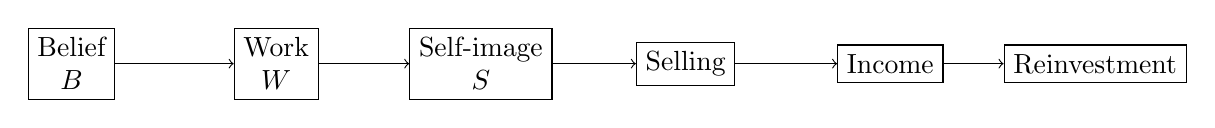
\begin{tikzpicture}[x=1cm,y=1cm]
\node[draw, align=center] (b) at (0,0) {Belief\\$B$};
\node[draw, align=center] (w) at (2.6,0) {Work\\$W$};
\node[draw, align=center] (s) at (5.2,0) {Self-image\\$S$};
\node[draw, align=center] (sell) at (7.8,0) {Selling};
\node[draw, align=center] (inc) at (10.4,0) {Income};
\node[draw, align=center] (re) at (13.0,0) {Reinvestment};

\draw[->] (b) -- (w);
\draw[->] (w) -- (s);
\draw[->] (s) -- (sell);
\draw[->] (sell) -- (inc);
\draw[->] (inc) -- (re);
\end{tikzpicture}
\caption{An editorial compression of the causal chain repeated throughout the interview.}
\end{figure}

\paragraph{Mechanism.}
The lecture adds three layers to this chain. First, work is said to beat competition because most competitors will not work at the necessary level. Second, psychology matters: reading people, understanding fear, and making contact are part of sales labor. Third, work ethic itself becomes a product. Sean explicitly says that in major distribution negotiations he sold his work ethic when capital and pedigree were missing.

\paragraph{Anecdote.}
The life-insurance story makes this vivid. Faced with a list of reasons that a carrier should not work with him, he does not claim unmatched expertise or deep reserves of capital. He says instead that what he has to sell is work ethic. That is a very sharp moment in the lecture, because it converts an internal trait into a commercial offer.

\begin{remark}
This section is not a measured psychological model. It is a transcript-backed mechanism. The arrows indicate narrative causation as the interview presents it, not coefficients estimated from data.
\end{remark}

\section{Selling Yourself, Selling Truth, and Building Trust}

After the sales mechanism comes the next question: if many products are substantially similar, what exactly are we selling? The lecture answers by shifting the sale from product-difference to person-difference. In life insurance, in waste management, and in other service businesses, Sean insists that the product class is often close to commoditized. The differentiator is the trusted operator.

\paragraph{Claim.}
The lecture's answer is not egoistic self-promotion. In fact, it repeatedly warns that ego destroys duplication. To sell oneself well is to present confidence and humility together: confidence about what one can do, humility about what one cannot do.

\paragraph{Mechanism.}
Trust is operationalized in small repeatable acts. The lecture gives several:
\begin{enumerate}
\item change the voicemail daily with one's own voice;
\item return calls and messages within twenty-four hours;
\item do what one says one will do;
\item ask for permission to be brutally honest;
\item then state the real implications of action and inaction.
\end{enumerate}

This is not presented as branding fluff. It is presented as a way to solve what the lecture calls the client's central fear: that the seller will lie.

The trust sequence is simple:
\begin{enumerate}
\item establish that honesty will be the rule;
\item obtain explicit permission to speak plainly;
\item present the product, the price, and the consequences of refusal;
\item let truth, not theatrical pressure, do the work.
\end{enumerate}

A small explicit example is given in the transcript. A product costs \$720 per month because the buyer's health history is poor. The important pedagogical point is not the number by itself. It is that the number becomes easier to present once the parties have agreed to live inside the truth rather than in mutual avoidance.

The lecture also introduces a second, quieter rule here: relationships are built by doing things one does not strictly have to do. In Sean's language, the ``currency'' of a relationship is often found precisely in the unnecessary act. That is how the sale of the person accumulates over time.

\section{Scaling, Patience, and the Three-Legged Stool}

The lecture next widens from personal selling to organizational design. Sean moves from his own behavior into the structure of a business that can grow without collapsing into ego, fragility, or premature extraction.

A quantitative anchor is supplied when he reports the scale of the life-insurance business:
\begin{equation}
R_{2023} = \$752{,}000{,}000.
\end{equation}
The point of the figure is not celebration alone. It is tied to distribution, infrastructure, and leadership depth. The company did not reach that scale by one person wearing every hat.

\paragraph{Anecdote.}
The lecture's most useful organizational embarrassment is the moment when a prospective buyer asks for his C-level executives and he realizes that, in practice, he is all of them. That becomes a diagnosis. One may be the chief executive and still be unqualified to function as the chief financial officer or the technology head. Scaling therefore requires both humility and hiring.

\paragraph{Mechanism.}
Delegation is not merely a matter of saving time. It is a matter of preserving role quality. The lecture's underlying rule is: do not confuse control with competence. Bringing in finance, technology, and infrastructure people frees the founder to do the things at which he is actually strong.

The companion financial lesson comes through Arthur Blank and later mentors. Feed the business. Do not starve it. Accept small margins early if the structure is sound. Let ``a little bit of a lot'' become enough.

\begin{definition}[Three-Legged Stool]
A business decision \(D\) is acceptable only if it is good for the client, good for the worker or agent, and not harmful to the company.
\end{definition}

In compact form,
\begin{equation}
D \text{ is admissible} \iff (D \text{ serves the client}) \land (D \text{ serves the worker}) \land \neg(D \text{ harms the firm}).
\end{equation}

\begin{table}[h]
\centering
\begin{tabular}{|l|p{8.2cm}|}
\hline
Leg & Interpretation in the lecture \\
\hline
Client & the product, service, or price must genuinely work for the buyer \\
\hline
Worker / agent & the people carrying the business must be able to win with the decision \\
\hline
Company & the choice cannot destroy long-term sustainability \\
\hline
\end{tabular}
\caption{Sean's ``three-legged stool'' as a decision filter.}
\end{table}

This is one of the clearest quasi-formal rules in the entire interview. It also ties directly to his refusal to take all the credit. A company can be starved not only of money but of dignity. If the founder monopolizes praise, then second- and third-level leaders never mature. The interview is very explicit here: companies often fail because credit, not cash, is hoarded.

\section{Debt, Bankruptcy, and Wealth Architecture}

The lecture now turns from business operations to capital structure. Sean opposes what he calls learned middle-class behavior with a wealth-building mindset. The first mindset saves obediently, fears debt, and aims at bill payment. The second asks what capital can do when it is deployed intelligently.

\paragraph{Anecdote.}
Bankruptcy is presented not as an unqualified disaster but as a brutal education. The crucial move comes immediately afterward: rebuild credit, borrow again, and use access to capital as an instrument of opportunity. Within about a year and a half, he reports obtaining
\begin{equation}
L_{\text{LOC}} = \$1{,}000{,}000
\end{equation}
from a local bank.

\paragraph{Claim.}
The central leverage rule is expressed plainly:
\begin{equation}
r_{\text{deploy}} > r_{\text{borrow}}.
\end{equation}
That is the entire moral logic of his defense of debt. If borrowed money costs less than the return one can reliably produce with it, then debt is not merely tolerable; it is useful.

He gives a stylized version later:
\begin{equation}
r_{\text{borrow}} \approx 3\% < 8\% \approx r_{\text{deploy}}.
\end{equation}
Again, this is not a formal investment memorandum. It is an interview shorthand for why cheap money is attractive to someone who believes he can put it to work.

\paragraph{Worked Example: Hard Money.}
The clearest explicit financing example in the lecture is the hard-money loan:
\begin{align}
L_{\text{hard}} &= \$200{,}000,\\
r_{\text{hard}} &= 12\%.
\end{align}
If we compute only the stated six-month interest burden, we get
\begin{equation}
\text{six-month interest} \approx 0.12 \cdot \frac{1}{2} \cdot \$200{,}000 = \$12{,}000.
\end{equation}
The transcript then adds ``10 points every six months.'' If we use the standard finance convention that one point is one percent of principal, then
\begin{equation}
\text{points over six months} \approx 0.10 \cdot \$200{,}000 = \$20{,}000.
\end{equation}
So the six-month financing cost, before repayment of principal, is roughly
\begin{equation}
\$12{,}000 + \$20{,}000 = \$32{,}000.
\end{equation}

\begin{remark}
This is a cautious reconstruction, not a transcript-native APR calculation. The lecture's point is qualitative and practical: once interest and points are combined, the hurdle is high. Such money makes sense only if the project return is comfortably above the financing cost.
\end{remark}

The lecture's polemical edge comes from this contrast. Some people fear all debt because they see only obligation. Sean sees optionality. The same borrowed capital that terrifies one person becomes a lever for another. He therefore reframes debt as a tool whose value depends on the user's commercial competence.

\section{Escaping Poverty, Surviving the Storm, and the Blueprint}

The final movement of the lecture brings the argument back to the beginner. It first returns to poverty, then passes through crisis, and finally compresses the whole interview into a practical blueprint.

\paragraph{Claim.}
Sean rejects the slogan that the poor must remain poor. His alternative is not abstract optimism. It is a sequence: get around people who make money, ask questions, learn sales, recruit, teach, and scale. Sales is named the great equalizer because entry cost is low relative to capital-heavy ownership, while the upside expands once distribution is built.

\paragraph{Mechanism.}
The lecture's poverty-escape mechanism can be summarized as follows:
\begin{enumerate}
\item begin with low capital and limited network;
\item enter sales, where effort substitutes for inherited assets;
\item work until self-image improves;
\item use sales income to fund businesses or agency growth;
\item recruit and teach others;
\item convert individual effort into distribution.
\end{enumerate}

The crisis material sharpens this further. In both the temporary restraining order episode and the waste-management incinerator disaster, the lecture narrows chaos into a smaller action set. This is one of the cleanest procedural ideas in the interview.

\begin{definition}[Control Partition]
In a crisis, divide the present mess into two sets: the things that can be acted upon now and the things that cannot.
\end{definition}

We may write that partition as
\begin{equation}
\text{Problem set} = \mathcal{C} \sqcup \mathcal{N},
\end{equation}
where \(\mathcal{C}\) is the control set and \(\mathcal{N}\) is the noise set. The action rule is then
\begin{equation}
\text{Act on } \mathcal{C}, \qquad \text{do not spend the day living in } \mathcal{N}.
\end{equation}

This is exactly how the lecture handles adversity. The court order arrives; he asks what happens if he violates it. The incinerator burns; he asks where the trash can go, who owns the landfills, who knows whom, and what can be negotiated. The point is not that the environment is fair. The point is that action begins only after the controllable slice has been isolated.

The closing blueprint returns to visible symbols of wealth, including the private jet. Here the lecture inserts one final quantitative caution:
\begin{equation}
C_{\text{jet,idle}} \gtrsim \$150{,}000/\text{month}.
\end{equation}
Buying is not the main difficulty; carrying cost is. This is a fitting closing number, because it captures the lecture's whole view of wealth. Wealth is not mere acquisition. It is the power to support and govern expensive structures over time.

The final advice therefore compresses the chapter rather than changing it. Ask better questions. Find a good attorney and accountant early. Seek capital from local banks and from people who can see value in you. Learn to talk to different classes of people in the same day. Accept that discomfort often marks growth. Be teachable. Do not be egotistical. And, above all, become good at sales.

\section{Summary}

The lecture begins with a billion-dollar promise and ends with a beginner's blueprint. In between, it constructs a distinct commercial philosophy. We first learn to distrust appearances and ask for paper. We then learn that sales is not merely persuasion but a chain linking belief, work, self-image, trust, and distribution. Next we learn that wealth is built less by early extraction than by feeding the business, sharing credit, and making decisions that satisfy the client, the worker, and the firm at once. Finally, we learn that debt, crisis, and discomfort are not to be romanticized, but neither are they to be feared in the abstract. They are to be handled with judgment, with structure, and with the stubborn discipline of doing the next controllable thing.